\chapter{Implementacija}
U ovom poglavlju se objašnjava arhitektura aplikacije u kojoj je implementiran model detekcije objekata. 
Model detekcije objekata pomoću konvolucijskih neuronskih mreža bit će implementiran za 
operacijski sustav Android. Koristit će se model u Tensorflow lite obliku, koji je je izveden iz Tensorflow modela.
Aplikaicija je pisana u radnom okviru Flutter koristeći programski jezik Dart. 
Više o samim tehnologijama će biti rečeno u nastavku.

\section{Tehnologije}
Za implementaciju modela detekcije objekata korištene su različite tehnologije, bez kojih bi postupak bio značajno otežan i 
skloniji pogreškama.
\subsection{Tensorflow}
Tensorflow je Google-ova biblioteka otvorenog koda. Služi kao sučelje za uporabu algoritama strojnog i dubokog učenja, te implementaciju
istih. Tensorflow omogućuje pisanje koda visoke razine, te je na korisniku da se koncentrira na izgled modela i slojeve koji su zastupljeni u samom
modelu, dok će sam Tensorflow brinuti za ostale postupke koji se događaju u pozadini. Širok je spektar proizvoda koji se mogu razvijati pomoću
Tensorflowa, kao što su: 
\begin{itemize}
    \item Detekcija govora
    \item Ekstrahiranje geografskih informacija
    \item Procesuiranje prirodnog govora
\end{itemize}
Fleksibilna arhitektura Tensorflow-a omogućuje korisniku razvoj i pokretanje modela
na procesoru, grafičkoj kartici, pa čak i TPU (Tensor processing unit).
Mobilna inačica Tensorflowa naziva se Tensorflow Lite. 
Razlog razvoja ove inačice bila je sve veća količina podataka koje su mobilni uređaji 
mogli pohraniti, ali i sve veća procesorska snaga. Milijuni korisnika diljem svijeta svakog 
trenutka koriste svoje mobilne uređaje za neke određene zadatke, te nije praktično imati model na 
udaljenom poslužitelju kojemu se pristupa putem mobilnog uređaja. Zato je Tensorflow Lite značajan za daljnji razvoj i 
implementaciju modela dubokog i strojnog učenja, jer eliminira potrebu za spajanjem na poslužitelj i ubrzava postupak dobivanja
rezultata od modela. 

\begin{figure}[htb]
    \centering
    
\includegraphics[width=10cm]{img/tensorflow.png}
    \caption{Tensorflow je jedna od najpoznatijih biblioteka otvorenog koda}
    \label{Tensorflow}
\end{figure}


\subsection{Flutter}
Razvoj mobilnih aplikacija u današnje doba od velike je važnosti zbog sve veće globalne potražnje. Dvije mobilne platforme koje imaju najveći udio na 
tržištu su Apple-ov IOS, te Google-ov Android. Vještine u izradi aplikacija i sustava za ove platforme izrazito je traženo, ali problem s kojim se mnogi
susreću je potraga za programerima za IOS i Android, zbog toga što se ne koriste isti jezici i radni okviri za razvoj istih. 
Radni okvir Flutter nastoji riješiti ovu poteškoću tako što nudi mogućnost kompajliranja koda i za IOS i za Android, ali sve iz iste baze koda. 
Nastao je sa strane Google-a 2017. godine, kada je jedino mogao kompajlirati kod za Android operativni sustav. 

Programski jezik koji se koristi za razvoj unutar ovog okvira naziva se Dart, koji je isto razvijan u Google-u. 
Glavna komponenta u Flutter-u jesu "Widgeti", koji služe za prikaz elemenata na ekranu. Dva skupa ovih komponenti koje postoje unutar radnog 
okvira su Material Design (Android), te Cupertino (IOS).\newline
U najnovijoj inačici Fluttera postoji mogućnost pokretanja aplikacija kao web aplikacije, iako 
je ova mogućnost i dalje u beta razvoju. 

\begin{figure}[htb]
    \centering
    
\includegraphics[width=10cm]{img/flutter.png}
    \caption{Flutter omogućuje razvoj aplikacija za više platformi}
    \label{Flutter}
\end{figure}


\section{Model}
Model koji se koristi za implementaciju metode detekcije objekata je SSD MobileNet.
Razlog za ovaj model jest mogućnost treniranja modela pomoću transfer learninga na Google-ovom oblaku, što je detaljnije pojašnjenu u nastavku.
SSD MobileNet inačica je običnog SSD-a prilagođena za izvođenje na mobilnim uređajima.
Ovakva arhitektura modela daje rezultate brže i točnije od YOLO modela, a isto tako je i točnija od 
sporijih arhitektura koje koriste tehniku pretpostavljenih regija, poput Brzog R-CNN. \citep{DBLP:journals/corr/LiuAESR15}

Na slici ~\ref{SSD model} moguće je vidjeti kako SSD generira okvire oko objekata. Za treniranje ovog modela potrebno je unijeti sliku
te "groud truth" okvire kako bi model raspoznao objekte od pozadine. Model sadrži predefinirane okvire različitih veličina pomoću kojih 
se dolazi do mape značajki. Dimenzije mape značajki označavaju koliko točaka od predefiniranih okvira se poklapa ili nalazi unutar danih "ground truth" okvira.
Na primjer, ako se izvede mapa značajki 8x8, to znači da su 2 predefinirana okvira unutar "ground truth" okvira jer svaki ima 4 točke. 

\begin{figure}[htb]
    \centering
    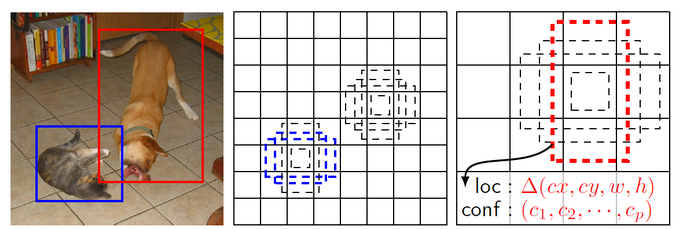
\includegraphics[width=10cm]{img/SSD.png}
    \caption{1. slika označava ulaz sa "groud truth" okvirima. 2. Slika označava mapu značajki koja je 8x8. 3. Slika označava mapu značajki koja je 4x4}
    \label{SSD model}
\end{figure}


\section{Implementacijski postupak}
Postupak treniranja i implementiranja modela značajno je pojednostavila činjenica da Google u ponudi ima širok spektar različitih modela koji su istrenirani
do određene točke, gdje se dalje mogu modificirati i istrenirati po potrebi i samim time uštedjeti i na računalnim i vremenskim resursima. 
Implementacija sadržava gore navedene tehnologije bez kojih krajnji proizvod ne bi bio ni približno stabilan te robustan kao što je sada. 

\subsection{Izgled skupa podataka i pohrana}
Za početak je bilo potrebno odrediti razrede koje će model moći prepoznati i pronaći odgovarajući skup fotografija koje odgovaraju razredima. Ova implementacija može raspoznati pasmine pasa i mačaka. 
Preuzeti skup slika sadrži oko 7400 slika mačaka i pasa. Što se konkretno tiče broja različitih razreda koje ovaj model može prepoznati, unutar skupa se nalaze 37 razreda od kojih je podjednak
broj za pse i mačke. Svaka slika unutar skupa sa sobom ima odgovarajuću anotaciju koja daje informaciju o koordinatama okvira koji omeđuje životinju na slici. 

Nakon što je skup slika preuzet potrebno ga je pretvoriti u odgovarajući format (TFRecord) koji je prikladan za daljnju analizu, što je bilo moguće ostvariti pomoću skripti koje se mogu preuzeti iz Googleovog repozitorija na githubu.
Generiranje TFRecord-a daje kao rezultat dva skupa datoteka, jedan je skup koji se koristi za treniranje, dok je drugi skup koji se koristi za validaciju. Kako bi model mogao točno klasificirati objekte na pojedinim lokacijama generirana
je datoteka s labelama.

\begin{figure}[ht]
    \centering
    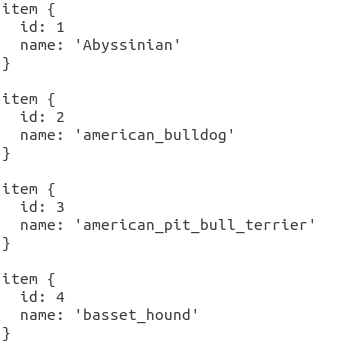
\includegraphics[width=8cm]{img/pet_labels.png}
    \caption{Odsječak iz datoteke s labelama korištenim prilikom treniranja}
    \label{Pet labels}
\end{figure}

Kao pomoć prilikom pohranjivanja datoteka iskorištena je Google-ova usluga u oblaku, koja omogućuje pohranjivanje i izvođenje različitih zadataka bez korištenja vlastitih resursa. 
Kako bi sve funkcioniralo, prvo se treba postaviti novi "bucket" u kojem se mogu pohranjivati sve datoteke i rezultati treniranja. Za postavljanje navedenog direktorija korišten je gsutil sučelje kroz 
komandnu liniju. Korištenje ovog sučelja jednostavno je i omogućuje brzo postavljanje novog projekta i prostora za pohranu. Za potrebe ovog rada korištena je probna inačica koja traje 365 dana, te nudi 300 USD na korištenje. 
Unutar probne inačice se nalaze sve potrebne komponente za kvalitetno provođenje treniranja i pohrane podataka.

\begin{figure}[htb]
    \centering
    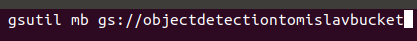
\includegraphics[width=10cm]{img/Gsutil.png}
    \caption{Postavljanje novog bucketa unutar projekta pomoću komandne linije}
    \label{Gsutil}
\end{figure}

\subsection{Sučelja i alati}
Nakon konfiguracije projekta na oblaku potrebno je instalirati Tensorflow Object Detection API koji u sebi sadrži brojne skripte i konfiguracijske datoteke korištene prilikom postavljanja okruženja za treniranje i evaluaciju. 
Za lakšu instalaciju paketa potrebnih za rad sučelja preuzet je upravitelj paketima anaconda. Anaconda je veoma praktičan alat koji se koristi u znanstvenom računanju i služi za jednostavnije upravljanje i implementaciju paketa. 
Po instalaciji alata kreirano je novo virtualno okruženje u kojem su bili naknadno preuzeti paketi. Tensorflow Object Detection API bio je preuzet sa službenog github repozitorija te je pomoću testne skripte bio konfiguriran.
Uz ovo sučelje instalirano je i sučelje COCO. COCO je veliki skup fotografija koji se koristi za razne zadatke poput detekcije objekata, segmentacije i drugih.

Konfiguracija svih potrebnih direktorija i sučelja veoma je bitno na početku napraviti kako treba, jer kasnije može doći do neželjenih poteškoća prilikom implementacije. Više o ovim poteškoćama i mogućim rješenjima mogu se nači u dodatku A.

\subsection{SSD Mobilenet}
Ograničenost vlastitih računalnih i vremenskih resursa zahtjevaju preuzimanje treniranog modela koji ima postavljene parametre i arhitekturu, te koristeći se tehnikom 
tranzitivnog učenja trenirati model. Na službenom github repozitoriju\footnote{\url{https://github.com/tensorflow/models/blob/master/research/object_detection/g3doc/detection_model_zoo.md}}
postoje mnogi različiti modeli koji se mogu koristiti za tranzitivno učenje. Ovaj model \footnote{\url{http://download.tensorflow.org/models/object_detection/ssd_mobilenet_v1_0.75_depth_quantized_300x300_coco14_sync_2018_07_18.tar.gz}}
je izabran zbog kompatibilnosti izvođenja na TPU, koji omogućuje brže treniranje. Nakon preuzimanja modela kontrolne točke bile su kopirane u isti direktorij gdje se nalaze i datoteke koje služe za treniranje. 
Kako se koristi pretreniran model s konfiguriranom arhitekturom i parametrima potrebno je, osim postavljanja kontrolnih točaka, postaviti konfiguracijsku datoteku u kojoj se zapisuju podaci bitni za daljnje treniranje i
evaluaciju istreniranog modela. U toj konfiguracijskoj datoteci postavljaju se vrijednosti poput broja razreda, broja testnih primjeraka i funkcije za računanje stope učenja. 
Odsječak iz ove datoteke dan je u nastavku.

\begin{figure}[htb]
    \centering
    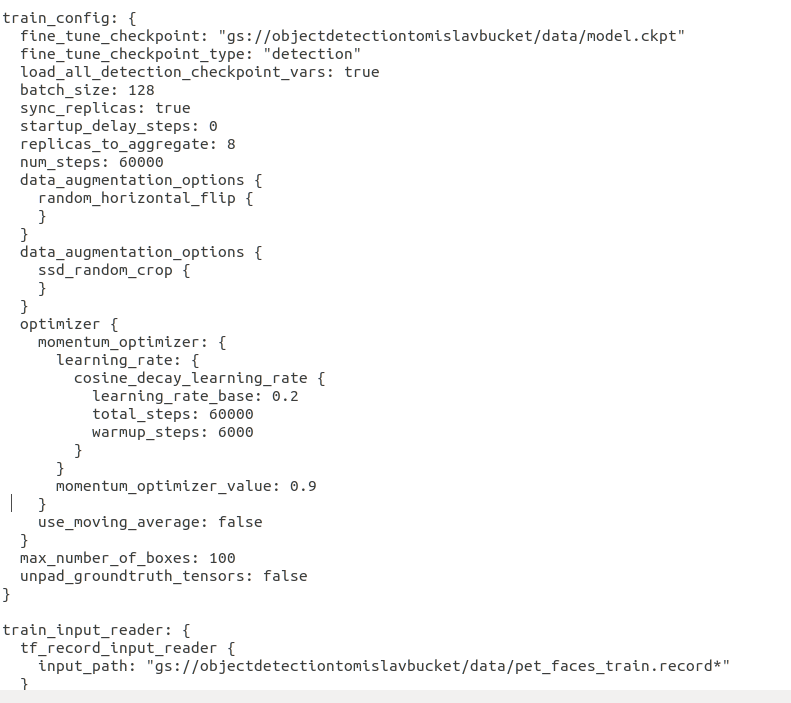
\includegraphics[width=10cm]{img/pipeline.png}
    \caption{Odsječak iz konfiguracijske datoteke u kojem se postavlja konfiguracija za treniranje}
    \label{Pipeline}
\end{figure}

\begin{figure}[htb]
    \centering
    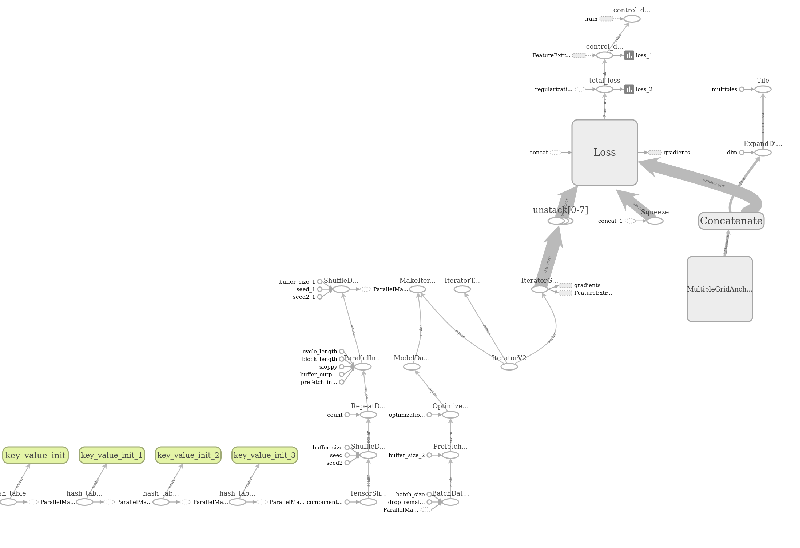
\includegraphics[width=10cm]{img/izgled-modela.png}
    \caption{Graf tensorflow modela korištenog prilikom treniranja}
    \label{TF-model}
\end{figure}


\subsection{Treniranje}
Treniranje ovog modela zahtjeva prolazak kroz sve primjerke za treniranje i uspoređivanje pretpostavljenih okvira s stvarnim okvirima oko objekata. Budući da se treniranje odvija na oblaku 
nije bilo potrebno koristiti vlastite računalne resurse, što je znatno olakšalo razvoj. Gsutil sučelje putem komandne linije čini proces stvaranja novog treninga nad modelom 
jednostavno, međutim potrebno je prethodno konfigurirati sve datoteke kako bi cijeli postupak bio što efikasniji. Za potrebe pokretanja novog postupka treniranja napisana je vlastita
pomoćna skripta koja je dostupna u repozitoriju ovoga rada. Skripta služi kako bi se jednostavnije mogle postaviti putanje do svih potrebnih datoteka i direktorija. Također, unutar
skripte su navedene potrebne zastavice koje su nužne kako bi se trening izvršio. 

\begin{lstlisting}[language=bash, tabsize=2]
    #!/usr/bin/bash
    ...
    conda activate tensorflow_obj_detection
    cd ~/Tomo/Faks/Zavrsni-rad/model/models/research
    
    JOB= ...
    gcloud ai-platform jobs submit training $JOB \
    --job-dir=$JOB_DIR  \
    --packages $PACKAGES --module-name $MODULE_NAME_TPU \
    --runtime-version $RUNTIME_VERSION \ 
    --scale-tier $SCALE_TIER_TPU \
    $REGION $BLANK $TPU_ZONE \
    --model_dir=$MODEL_DIR \ 
    --pipeline_config_path=$PIPELINE_CONFIG_PATH
\end{lstlisting}

Kako bi sve moglo raditi, potrebno se prvo pozicionirati u "research" direktorij unutar tensorflow object detection API koji je prethodno preuzet i instaliran, jer se u njemu nalaze potrebne skripte i paketi nužni za 
rad. Za pokretanje treninga potrebno je postaviti direktorij treninga, tj. direktorij u koji se spremaju rezultati treniranja. Isto tako, treniranje se ne bi moglo izvršiti 
bez specificiranja paketa koji se koriste (više o konfiguraciji paketa bit će u repozitoriju), kao ni inačice tensorflowa koja se koristi prilikom izvođenja računskih operacija.

Prilikom treniranja pogreške prilikom klasifikacije objekata na slici su se relativno brzo smanjili, najvećim djelom zbog toga što se koristi konfigurirani model. Model nakon 20 tisuća koraka
nema znčajnijih promjena, tako da se može i smanjiti broj koraka treniranja kako bi se uštedjelo na računalnim i vremenskim resursima. Ovakvi kompormisi između dostupnih resursa i točnosti ili smanjenju
gubitaka nužni su kako bi se moglo doći do što kvalitetnijeg proizvoda s najmanjim mogućim ulogom.

\begin{figure}[htb]
    \centering
    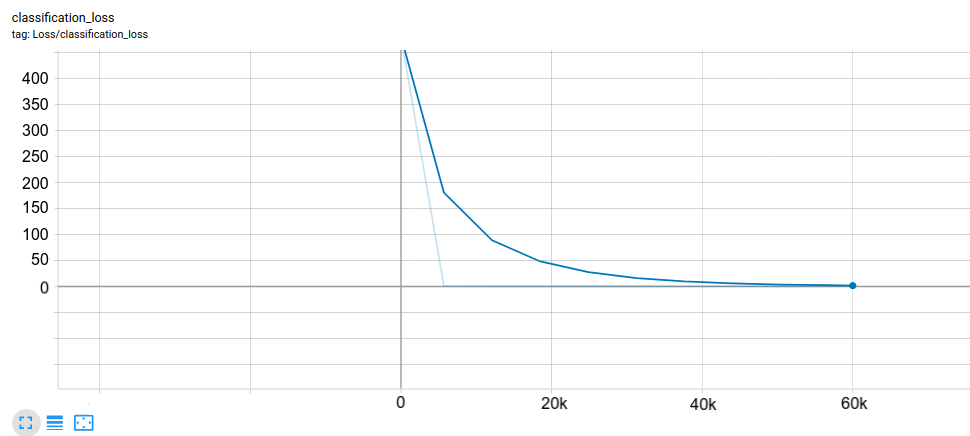
\includegraphics[width=12cm]{img/class-loss.png}
    \caption{Pogreška prilikom klasifikacije tokom treniranja}
    \label{Class-Loss}
\end{figure}


\begin{figure}[htb]
    \centering
    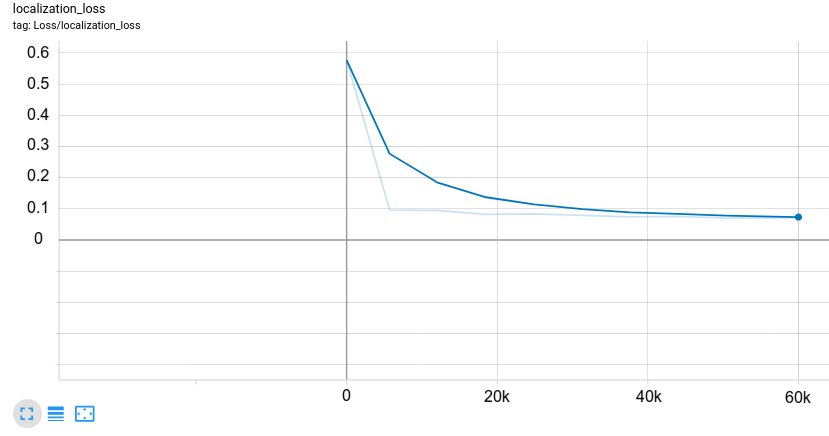
\includegraphics[width=12cm]{img/local-loss.png}
    \caption{Pogreška prilikom lokalizacije tokom treniranja}
    \label{Local-Loss}
\end{figure}

Pogreške u lokalizaciji također moraju biti praćene, jer kvalitetna detekcija objekata zahtijeva točnost i klasifikacije i lokalizacije objekata. Lokalizacaija objekata prilikom treniranja
ima očekivan pad pogreške, isto kao što ima i klasifikacija. Kod lokalizacije također nakon 20000 tisuća koraka nema značajnijeg pada postotka pogreške prilikom treniranja. 
Postupak treniranja unutar googleovog oblaka trajao je nešto manje od 2 sata, velikim djelom što je treniranje izvođeno na već treniranom modelu, ali isto tako što se koristio TPU. 

\subsection{Validacija}
Kako bi se moglo utvrditi točnost istreniranoga modela, potrebno je izvšiti validaciju nad testnim primjercima. Kao i kod treniranja, za validaciju se koristi google-ov oblak, ali se računanje izvodi
na GPU jer trenutno ne postoji mogućnost validacije na TPU. U istoj skripti koja se koristi za konfiguraciju putanja do potrebnih direktorija za treniranje nalazi se i kod koji pokreće potreban validacijski
postupak na oblaku. 

\begin{lstlisting}[language=bash, tabsize=2]
    #!/usr/bin/bash
    ...
    JOB_EVAL= ...
    gcloud ai-platform jobs submit training $JOB_EVAL \
    --job-dir=$JOB_DIR --packages $PACKAGES \
    --module-name $MODULE_NAME_GPU \
    --runtime-version $RUNTIME_VERSION \
    --scale-tier $SCALE_TIER_GPU $REGION $BLANK \
    --model_dir=$MODEL_DIR \
    --pipeline_config_path=$PIPELINE_CONFIG_PATH \
    --checkpoint_dir=$CHECKPOINT_DIR
\end{lstlisting}

Za validaciju nije potrebno promijeniti sve zastavice, već samo one koje određuju da se koristi GPU umjesto TPU. Validacija se izvršava paralelno s treniranjem i isto tako je bilo potrebno oko 
2 sata kako bi postupak bio gotov. Kod validacijskog postupka zapravo se provjera koliki je postotak poklapanja generiranog okvira od stvarnog okvira oko detektiranoga objekta, što se označava kao
mAP \engl{Mean Average Precision}. 

\begin{figure}[htb]
    \centering
    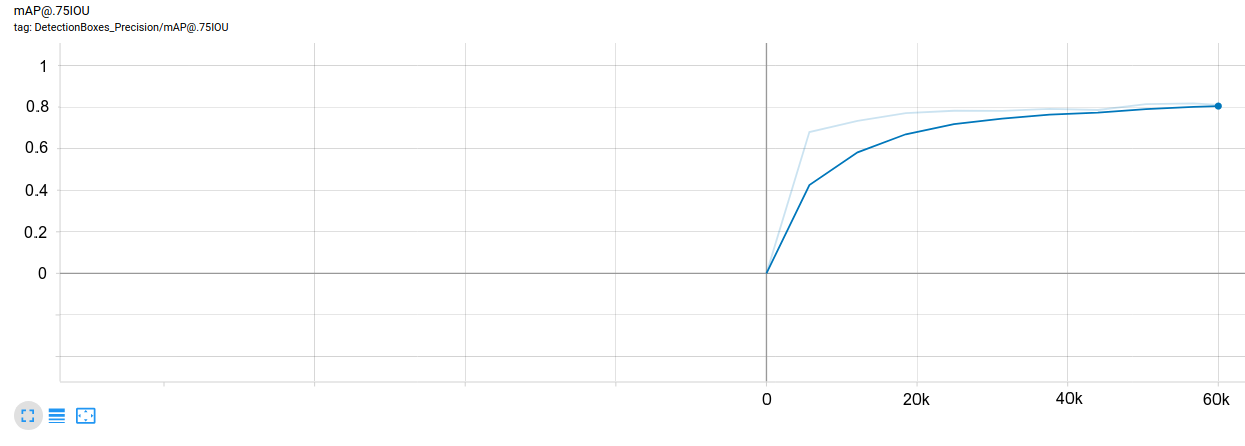
\includegraphics[width=14cm]{img/eval-mAP.png}
    \caption{Postotak poklapanja generiranog i stvarnog okvira prilikom validacije}
    \label{Eval-mAP}
\end{figure}

Računanje mAP vrijednosti radi se tako da se uzme IoU \engl{Intersect over Union}, tj. podijeli se presijek s unijom okvira. Ovakva vrsta validacije prilikom detektiranja objekata
dobar je pokazatelj preciznosti treniranog modela. Vizualni prikaz nalazi se na slici ~\ref{IoU}

\begin{figure}[htb]
    \centering
    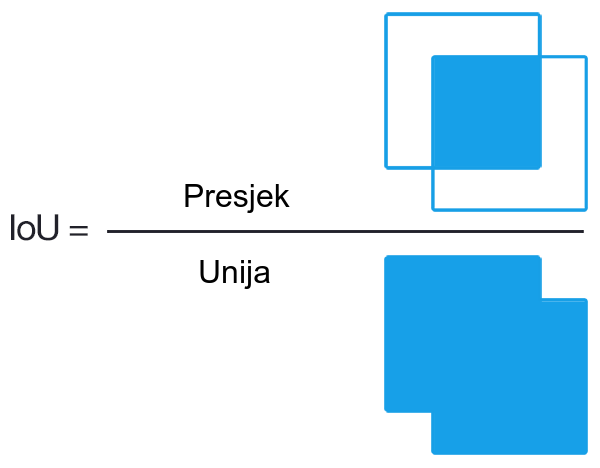
\includegraphics[width=10cm]{img/iou_equation.png}
    \caption{Omjer presjeka i unije koji služi za računanje mAP-a}
    \label{IoU}
\end{figure}

Iz grafa je vidljivo da se preciznost povećavala kako je model bio sve istreniraniji, što je u skladu s očekivanjima. Nakon cijelog postupka treniranja omjer presjeka i unije
od 0.75 je bio zastupljen u 80\% primjeraka. Postoje i drugi omjeri koji se mogu uzeti prilikom validacije, ali je omjer od 0.75 najrelevantiji za utvrđivanje preciznosti modela. 

\begin{figure}[htb]
    \begin{subfigure}{.8\textwidth}
        \centering
        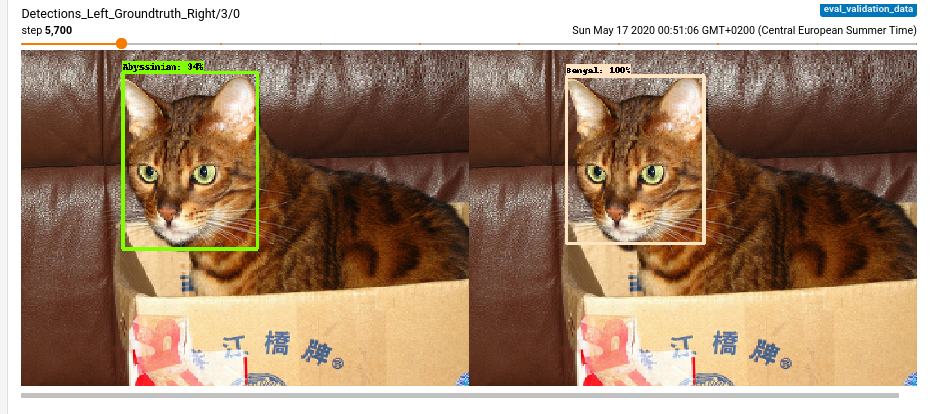
\includegraphics[width=.8\linewidth]{img/Cat-eval.png}
        \caption{Detekcija nakon 5700 koraka. Pogrešan razred}
        \label{Eval-cat}
    \end{subfigure}
    \begin{subfigure}{.8\textwidth}
        \centering
        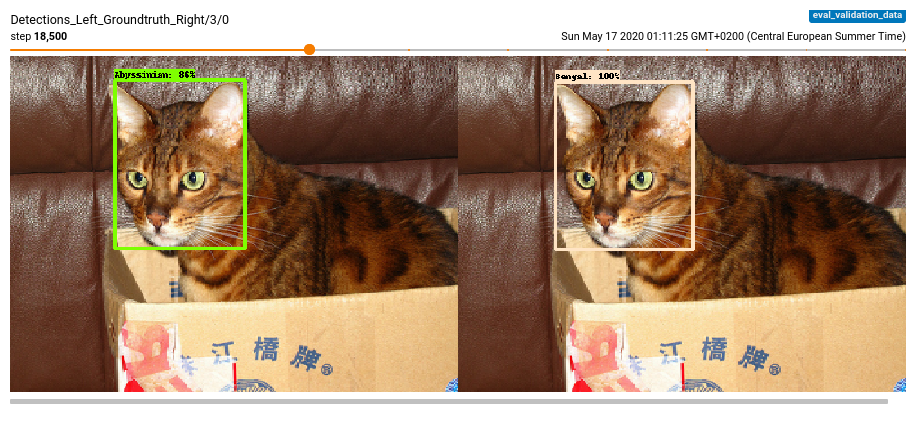
\includegraphics[width=.8\linewidth]{img/Cat-eval2.png}
        \caption{Detekcija nakon 18500 koraka. Pogrešan razred}
        \label{Eval-cat}
    \end{subfigure}
    \begin{subfigure}{.8\textwidth}
        \centering
        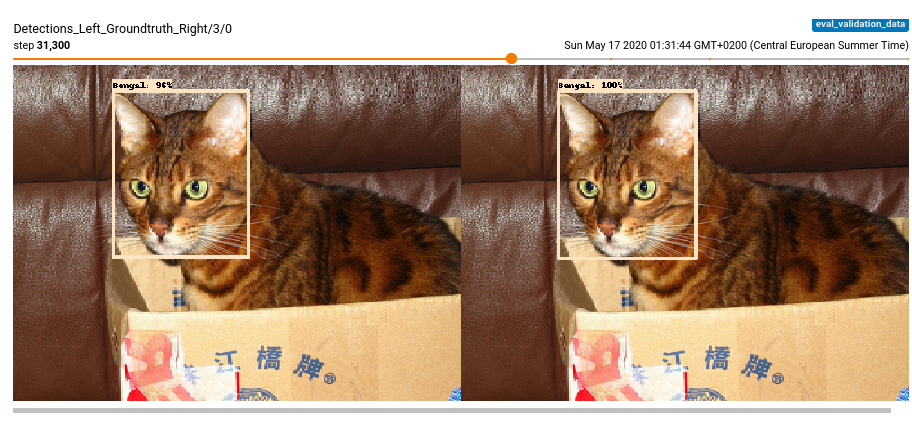
\includegraphics[width=.8\linewidth]{img/Cat-eval3.png}
        \caption{Detekcija nakon 31300 koraka. Točan razred}
        \label{Eval-cat}
    \end{subfigure}
\caption{Detekcija razreda tokom evaluacije u kojoj nakon 30000 koraka dolazi do točne klasifikacije}
\label{fig:CAT_Eval}
\end{figure}

\subsection{Mobilna aplikacija}
Nakon što je završilo treniranje i validacija modela, potrebno je premjestiti model u format za mobilne uređaje, drugim riječima u tensorflow lite. Kako bi se to moglo ostvariti potrebno je 
zamrznuti parametre trenutnog modela i pretvoriti njegov graf u zamrznuti graf \engl{frozen graph}. Kao i do sada, konvertiranje se odvija pomoću skripte u kojoj se navode potrebne putanje i poziva 
metoda tensorflow sučelja. Ovaj postupak odvija se unutar virtualnog okruženja koje je stvoreno u anacondi na samome početku, jer su u njemu konifgurirani potrebni paketi. Nakon konvertiranja u željeni format (.tflite umjesto .pb), potrebno 
je stvoriti novi flutter project. Kao razvojno okruženje koristi se Visual Studio Code, te su unutar njega instalirane potrebne ekstenzije za dart i flutter. 

Unutar samog projekta potrebno je dodati ovisnost \engl{dependency} o tflite paketu. Također je potrebno unutar assets direktorija dodati datoteku s labelama i sam model. 
Najprije je potrebno postaviti izgled zaslona po korisničkim zahtjevima. 


\begin{lstlisting}[tabsize=2]
    Widget _appBar() => AppBar(
        title: Text('Object detector'),
        centerTitle: true,
      );

  Widget _bottomNavigationBar() => BottomNavigationBar(
        items: const <BottomNavigationBarItem>[
          BottomNavigationBarItem(
              icon: Icon(Icons.camera_alt), title: Text('Static')),
          BottomNavigationBarItem(
              icon: Icon(Icons.videocam), title: Text('Dynamic')),
        ],
        currentIndex: _selectedIndex,
        selectedItemColor: Colors.tealAccent,
        onTap: _onItemTapped,
      );
}

\end{lstlisting}
